\subsection{Urządzenia IoT}

Urządzenia IoT są urządzeniami komputerowymi, z wbudowaną technologią do
bezprzewodowego dostępu do internetowego oraz przesyłu danych. Połączone urządzania komunikują
sie one między sobą, mogą być zdalnie monitorowane oraz kontrolowane. Wyposażone w odpowiednie
sensory znajdują wykorzystanie praktycznie we wszystkich typach urządzeń konsumenckich oraz
przemysłowych. Wydaje się naturalnym doposażanie takich urządzeń w coraz to lepsze podzespoły
pozwalające na uruchomienie coraz to bardziej wymagających obliczeniowo zadań. Obecnie produkuje się
wyspecjalizowane zestawy tworzone z myślą o konkretnych zastosowaniach i w tym o inferencji
modeli neuronowych. Do celów tej pracy przyjęto, że urządzenie końcowe powinno być wspierane
przez najpopularniejsze frameworki do tworzenia modeli neuronowych oraz powinno być do tego
wystarczająco wydajne. Zbiór platform został więc ograniczony do tych, które są w stanie
uruchomić system operacyjny Linux. W tabeli~\ref{table:device_comp} przedstawione zostało
porównanie najpopularniejszych urządzeń tego typu ze względu na czas inferencji wybranej sieci
neuronowej~\cite{BoardBenchmark} oraz ceny.

\begin{table}[h]
    \begin{tabular}{ccc}
   Platforma                            & Czas inferencji MobileNet~\cite{MobileNet} (ms) & Cena producenta \\[0.5ex] 
    \hline\hline
    Coral Dev Board                      & \num{15.7}           & \num{150}                  \\
    \hline
    NVIDIA Jetson Nano (TF)              & \num{276.0}          & \num{100}                  \\
    NVIDIA Jetson Nano (TF-TRT)          & \num{61.6}           & \num{100}                  \\
    \hline
    Raspberry Pi 4B (TF)                 & \num{263.9}          & \num{55}                   \\
    Raspberry Pi 4B (TF Lite)            & \num{82.7}           & \num{55}                   \\
    \hline
    Raspberry Pi + Coral USB Accelerator & \num{14.9}           & \num{130}                 
    \end{tabular}
    \caption{Porównanie urządzeń IoT.}
    \label{table:device_comp}
\end{table}

W tej pracy, wszelkie porównania zostaną wykonywane z użyciem platformy Raspberry Pi 4B w wersji z 4GB pamięci RAM. Wybór tego mikrokomputera został podjęty ze względu na jego największą powszechność wśród zarówno amatorów jak i profesjonalistów systemów wbudowanych oraz bardzo atrakcyjną cenę. Dzięki szybszemu złączu USB 3 platforma ta pozwala na rozszerzenie o zewnętrzne procesory obliczeniowe stworzone z myślą o inferencji modeli neuronowych takich jak ostatnio popularny Coral USB Accelerator. Niestety  względu na niewygodne ograniczenia co do możliwych do wykorzystania architektur sieci neuronowych oraz ograniczenie to frameworku TensorFlow w tej pracy ograniczymy sie do samego urządzenia Raspberry Pi 4 (rysunek \ref{fig:raspberry}).

\begin{figure}[h]
    \centering
    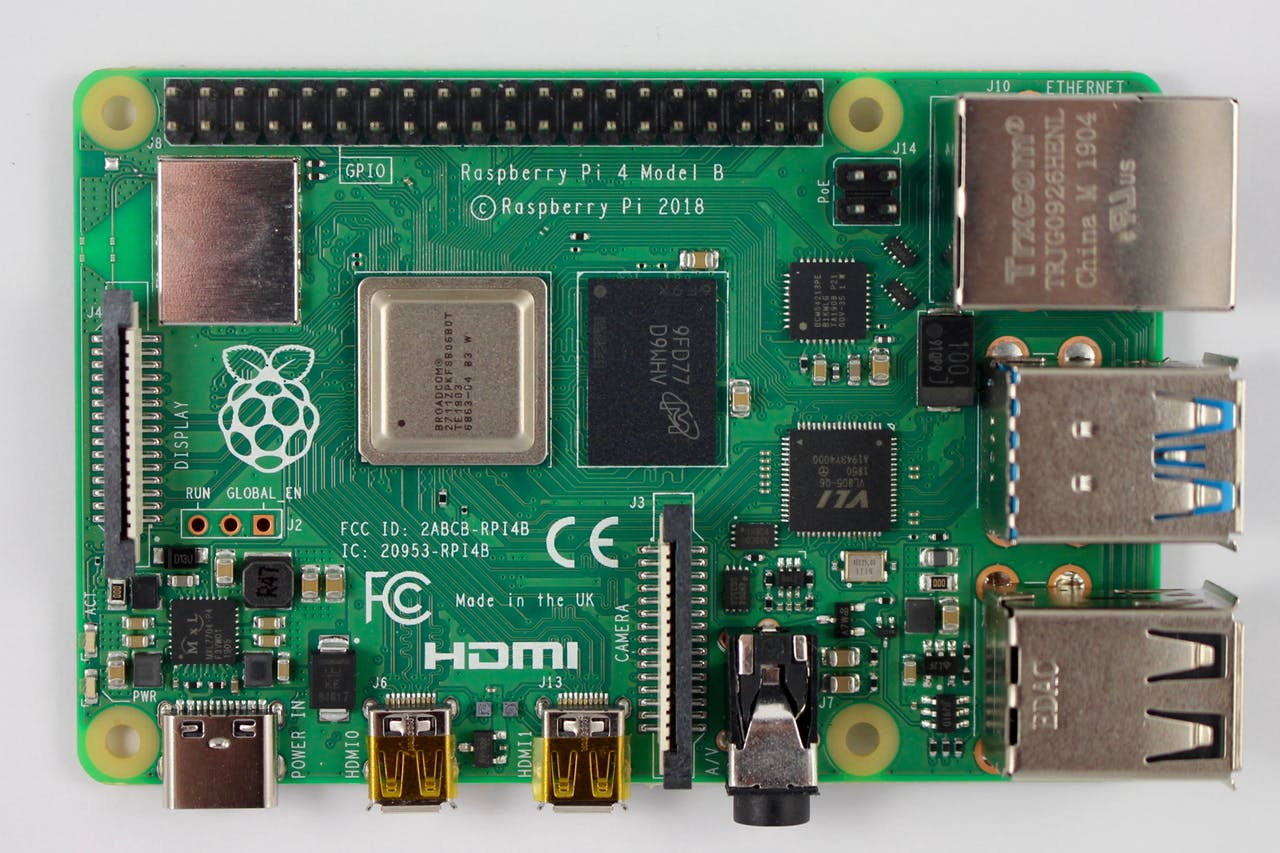
\includegraphics[width=0.8\linewidth]{img/rasberry.jpeg}
    \caption{Mikrokomputer Raspberry Pi 4B.}
    \label{fig:raspberry}
\end{figure}